\subsection{Comparison of NLP Models}
\label{sxn:nlp}

Within the past few years, nearly 100 open source, pretrained NLP DNNs based on the revolutionary Transformer architecture have emerged.
These include variants of BERT, Transformer-XML, GPT, etc.
The Transformer architectures consist of blocks of so-called Attention layers, containing two large, Feed Forward (Linear) weight matrices~\cite{Attn2017}. 
In contrast to smaller pre-Activation maps arising in Cond2D layers, Attention matrices are significantly larger.
In general, they have larger PL exponents $\alpha$.
Based on HT-SR Theory
(in particular, the interpretation of values of $\alpha \sim 2$ as modeling systems with good correlations over many size scales~\cite{BouchaudPotters03, SornetteBook}), 
this suggests that these models fail to capture successfully many of the information correlations in the data (relative to their size) and thus are substantially under-trained.
More generally, compared to CV models,
modern NLP models have larger weight matrices and display different spectral properties.

While norm-based metrics perform reasonably well on well-trained NLP models, they often behave anomalously on poorly-trained models.
For such models, weight matrices may display rank collapse, decreased Frobenius mass, or unusually small Spectral norms.
This may be misinterpreted as ``smaller is better.'' 
Instead, it should probably be interpreted as being due to a similar mechanism to how distillation can ``damage'' otherwise good models.
In contrast to norm-based metrics, PL-based metrics, including the Log $\alpha$-Norm metric and the Weighted Alpha metric, display more consistent behavior, even on less well-trained models.
To help identify when architectures need repair and when more and/or better data are needed,
one can use these metrics, 
as well as the decomposition of the Weighted Alpha metric ($\alpha\log\lambda_{max}$) into its PL component ($\alpha$) and its norm component ($\log\lambda_{max}$), for each layer.

Many NLP models, such as early variants of GPT and BERT, have weight matrices with unusually large PL exponents (e.g., $\alpha\gg 6$).
This indicates these matrices may be under-correlated (i.e., over-parameterized, relative to the amount of data).
In this regime, the truncated PL fit itself may not be very reliable because the Maximum Likelihood estimator it uses is unreliable in this range.
In this case, the specific $\alpha$ values returned by the truncated PL fits are less reliable, but having large versus small $\alpha$ is reliable.
If the ESD is visually examined, one can usually describe these $\mathbf{W}$ as in the \textsc{Bulk-Decay} or \textsc{Bulk-plus-Spikes} phase from HT-ST Theory~\cite{MM18_TR,MM19_HTSR_ICML}.
Previous work~\cite{MM18_TR,MM19_HTSR_ICML} has conjectured that very well-trained DNNs would not have many outlier $\alpha\gg 6$.
Consistent with this, more recent improved versions of GPT (shown below) and BERT (not shown) confirm~this.


\paragraph{OpenAI GPT Models.}

The OpenAI GPT and GPT2 series of models provide the opportunity to analyze two effects: increasing the sizes of both the data set and the architectures simultaneously; and training the same model with low-quality data versus high-quality data. 
These models have the ability to generate fake text that appears to the human to be real, and they have generated media attention because of the potential for their misuse.
For this reason, the original GPT model released by OpenAI was trained on a deficient data set, rendering the model interesting but not fully functional.  
Later, OpenAI released a much improved model, GPT2-small, which has the same architecture and number of layers as GPT, but which has been trained on a larger and better data set, making it remarkably good at generating (near) human-quality fake text.  
Subsequent models in the GPT2 were larger and trained to more data.
By comparing GPT2-small to GPT2-medium to GPT2-large to GPT2-xl, we can examine the effect of increasing data set and model size simultaneously, as well as analyze well-trained versus very-well-trained models.
By comparing the poorly-trained GPT to the well-trained GPT2-small, we can identify empirical indicators for when a model has been poorly-trained and thus may perform poorly when deployed.
The GPT models we analyze are deployed with the popular HuggingFace PyTorch library~\cite{huggingface}.


\begin{table}[t]
\small
\begin{center}
\begin{tabular}{|p{1in}|c|c|c|c|c|}
\hline
 Series  & \#   & $\langle\log\Vert\mathbf{W}\Vert_{F}\rangle$ & $\langle\log\Vert\mathbf{W}\Vert_{\infty}\rangle$ & $\hat{\alpha}$ & $\langle\log\Vert\mathbf{X}\Vert^{\alpha}_{\alpha}\rangle$ \\
\hline
GPT & 49 & 1.64  & 1.72 & 7.01 & 7.28 \\
GPT2-small & 49 & 2.04  & 2.54& 9.62 & 9.87 \\
%\hline
GPT2-medium & 98 & 2.08 & 2.58& 9.74 & 10.01 \\
GPT2-large & 146 & 1.85 & 1.99& 7.67 & 7.94 \\
GPT2-xl & 194 & 1.86 & 1.92 & 7.17 & 7.51 \\
\hline
\end{tabular}
\end{center}
\caption{Average value for the average Log Norm and Weighted Alpha metrics for pretrained OpenAI GPT and GPT2 models. 
Column \# refers to number of layers treated.  
Averages do not include the first embedding layer(s) because they are not (implicitly) normalized.  
GPT has 12 layers, with 4 Multi-head Attention Blocks, giving $48$ layer Weight Matrices, $\mathbf{W}$.
Each Block has 2 components, the Self Attention (attn) and the Projection (proj) matrices.  
Self-attention  matrices are larger, of dimension ($2304\times 768$) or ($3072\times 768$).
The projection layer concatenates the self-attention results into a vector (of dimension $768$).
This gives $50$ large matrices.
Because GPT and GPT2 are trained on different data sets, the initial Embedding matrices differ in shape.
GPT has an initial Token and Positional Embedding layers, of dimension $(40478\times 768)$ and $(512\times 768)$, respectively, whereas GPT2 has input Embeddings of shape $(50257\times 768)$ and $(1024\times 768)$, respectively. 
The OpenAI GPT2 (English) models are: GPT2-small, GPT2-medium, GPT2-large, and GPT2-xl, having $12$, $24$, $36$, and $48$ layers, respectively, with increasingly larger weight~matrices.
}
\label{table:nlp}
\end{table}


\paragraph{Average Quality Metrics for GPT and GPT2.}

We examine the performance of the four quality metrics (Log Frobenius norm, Log Spectral norm, Weighted Alpha, and Log $\alpha$-Norm) for the OpenAI GPT and GPT2 pretrained models.
See Table \ref{table:nlp} for a summary of results.
%
Comparing trends between GPT2-medium to GPT2-large to GPT2-xl,
observe that (with one minor exception involving the log Frobenius norm metric) all four metrics decrease as one goes from medium to large to xl.
This indicates that the larger models indeed look better than the smaller models, as expected.
GPT2-small violates this general trend, but only very slightly.
This could be due to under-optimization of the GPT2-small model, or since it is the smallest of the GPT2 series, and the metrics we present are most relevant for models at scale.
Aside from this minor discrepancy, overall for these well-trained models, all these metrics now behave as expected, i.e., there is no Scale Collapse and norms are decreasing with increasing~accuracy.

Comparing trends between GPT and GPT2-small reveals a different story. 
Observe that all four metrics increase when going from GPT to GPT2-small, i.e., they are larger for the higher-quality model (higher quality since GPT2-small was trained to better data) and smaller for the lower-quality model, when the number of layers is held fixed.
This is unexpected.
Here, too, we can perform model diagnostics, by separating $\hat{\alpha}$ into its two components, $\alpha$ and $\lambda_{max}$, and examining the distributions of each.
In doing so, we see additional examples of Scale Collapse and additional evidence for Correlation Flow.


\paragraph{Layer Analysis: Scale Collapse in GPT and GPT2.} 

We next examine the Spectral norm in GPT versus GPT2-small.
In Figure~\ref{fig:GPT-snorm-hist}, the poorly-trained GPT model has a smaller mean/median Spectral norm as well as, spuriously, many much smaller Spectral norms, compared to the well-trained GPT2-small.
This violates the conventional wisdom that smaller Spectral norms are better.
Because there are so many anomalously small Spectral norms, the GPT model appears to be exhibiting a kind of Scale Collapse, like that observed (in Figure~\ref{fig:resnet204D5L}) for the distilled CV models.
This demonstrates that, while the Spectral (or Frobenius) norm may correlate well with predicted test error, at least among reasonably well-trained models, it is not a good indicator of the overall model quality in general.
Na\"ively using it as an empirical quality metric may give spurious results when applied to poorly-trained or otherwise deficient~models. 


\begin{figure}[hbt!] %[t]
    \centering
    \subfigure[Log Spectral Norm ($\log\Vert\mathbf{W}\Vert_{\infty}$)]{
        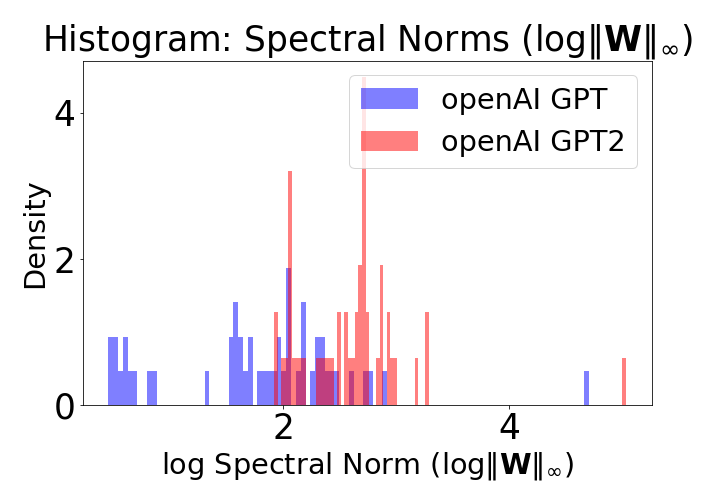
\includegraphics[width=5.5cm]{img/GPT-snorm-hist.png}

        \label{fig:GPT-snorm-hist}
       }
    \qquad
    \subfigure[PL exponent ($\alpha$)]{
      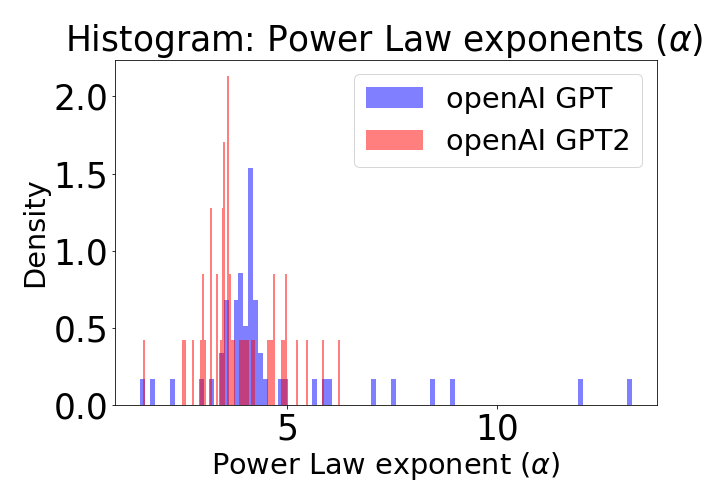
\includegraphics[width=5.5cm]{img/GPT-alpha-hist.png}
      \label{fig:GPT-alpha-hist}
       }
   \caption{Histogram of PL exponents 
           %($\alpha$) 
           and Log Spectral Norms 
           %($\log\Vert\mathbf{W}\Vert_{\infty}$) 
           for weight matrices from the OpenAI GPT and GPT2-small pretrained models.}
   
\label{fig:GPT-hist}
\end{figure}

\begin{figure}[hbt!] %[t]
    \centering
    \subfigure[Log Spectral Norm ($\log\Vert\mathbf{W}\Vert_{\infty}$)]{
        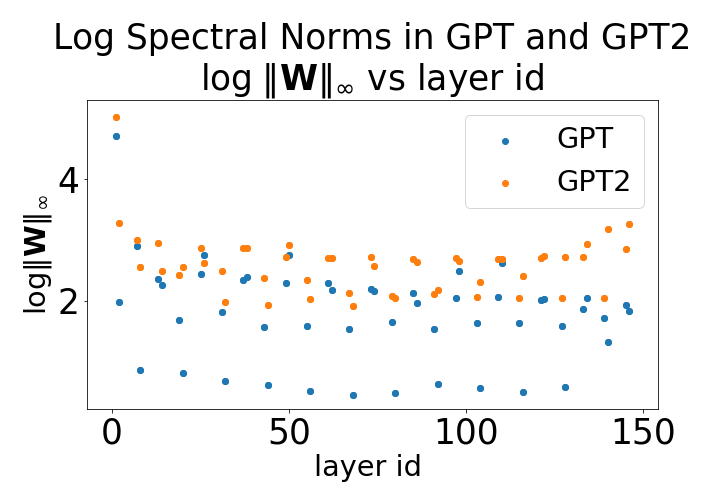
\includegraphics[width=5.5cm]{img/GPT-snorm-depth.png}
        \label{fig:gpt-snorm-layer}
    }
    \quad
    \subfigure[PL exponent ($\alpha$)]{
        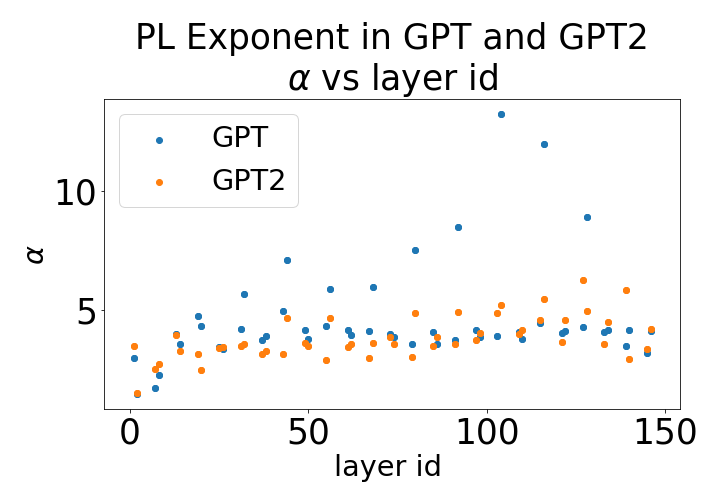
\includegraphics[width=5.5cm]{img/GPT-alpha-depth.png}
        \label{fig:gpt-alpha-layer}
    }
    \caption{%
             Log Spectral Norms 
             %($\log\Vert\mathbf{W}\Vert_{\infty}$) 
             (in (a)) 
             and 
             PL exponents 
             %($\alpha$) 
             (in (b)) 
             for weight matrices from the OpenAI GPT and GPT2-small pretrained models.  
             (Note that the quantities shown on each Y axis are different.)
             In the text, this is interpreted in terms of 
             Scale Collapse
             and 
             Correlation~Flow.
            }
    \label{fig:gpt-alpha-layers}
\end{figure}


Figure~\ref{fig:gpt-snorm-layer} shows the Spectral norm as a function of depth (layer id).
This illustrates two phenomenon.
First, the large value of Spectral norm (in Figure~\ref{fig:GPT-snorm-hist}) corresponds to the first embedding layer(s).
These layers have a different effective normalization, and therefore a different scale.
See the Supplementary Information
%~\ref{sxn:appendix} 
for details.
We do not include them in our computed average metrics in Table~\ref{table:nlp}.
%% and we do not include them in the histogram plot in Figure~\ref{fig:GPT-snorm-hist}.
Second, for GPT, there seems to be two types of layers with very different Spectral norms (an effect which is seen, but to a much weaker extent, for GPT2-small).
Recall that attention models have two types of layers, one small and large; and the Spectral norm (in particular, other norms do too) displays unusually small values for some of these layers for GPT.
This Scale Collapse for the poorly-trained GPT is similar to what we observed for the distilled ResNet20 model in Figure~\ref{fig:resnet204Dalpha}.
Because of the anomalous Scale Collapse that is frequently observed in poorly-trained models, these results suggest that scale-dependent norm metrics should not be directly applied to distinguish well-trained versus poorly-trained models. 


\paragraph{Layer Analysis: Correlation Flow in GPT and GPT2.} 

We next examine the distribution of $\alpha$ values in GPT versus GPT2-small.
Figure~\ref{fig:GPT-alpha-hist} shows the histogram (empirical density), for all layers, of $\alpha$ for GPT and GPT2-small.  
The older deficient GPT has numerous unusually large $\alpha$ exponents---meaning they are not well-described by a PL fit.
Indeed, we expect that a poorly-trained model will lack good (i.e., small $\alpha$) PL behavior in many/most layers.
On the other hand, the newer improved GPT2-small model has, on average, smaller $\alpha$ values than the older GPT, with all $\alpha\le6$ and with smaller mean/median $\alpha$.
It also has far fewer unusually-large outlying $\alpha$ values than GPT.
From this (and other results not shown), we see that $\bar{\alpha}$ 
from Eqn.~(\ref{eqn:alpha_bar}),
provides a good quality metric for comparing the poorly-trained GPT versus the well-trained GPT2-small.
This should be contrasted with the behavior displayed by scale-dependent metrics such as the Frobenius norm (not shown) and the Spectral~norm.
This also reveals why $\hat{\alpha}$ performs unusually in Table~\ref{table:nlp}.
The PL exponent $\alpha$ behaves as expected, and thus the scale-invariant $\bar{\alpha}$ metric lets us identify potentially poorly-trained models.
It is the Scale Collapse that causes problems for $\hat{\alpha}$ (recall that the scale enters into $\hat{\alpha}$ via the weights $\log\lambda_{max}$).

Figure~\ref{fig:gpt-alpha-layer} plots $\alpha$ versus the depth (layer id) for each model.
The deficient GPT model displays two trends in $\alpha$, one stable with $\alpha\sim 4$, and one increasing with layer id, with $\alpha$ reaching as high as $12$.
In contrast, the well-trained GPT2-small model shows consistent and stable patterns, again with one stable $\alpha\sim 3.5$ (and below the GPT trend), and the other only slightly trending up, with $\alpha\le 6$. 
These results show that the behavior of $\alpha$ across layers differs significantly between GPT and GPT2-small, with the better GPT2-small looking more like the better ResNet-1K from Figure~\ref{fig:resnet-alpha-layer}.
These results also suggest that smaller more stable values of $\alpha$ across depth is beneficial, i.e., that the Correlation Flow is also a useful concept for NLP~models.


\paragraph{GPT2: medium, large, xl.} 

We now look across series of increasingly improving GPT2 models (well-trained versus very-well-trained models), by examining both the PL exponent $\alpha$ as well as the Log Norm metrics.  
Figure \ref{fig:gpt2-histograms} shows the histograms over the layer weight matrices for fitted PL exponent $\alpha$ and the Log Alpha Norm metric. 
In general, and as expected, as we move from GPT2-medium to GPT2-xl, histograms for both $\alpha$ exponents and the Log Norm metrics downshift from larger to smaller values. 

From Figure~\ref{fig:gpt2-alpha-hist}, we see that
$\bar{\alpha}$, the average $\alpha$ value, decreases with increasing model size (XXX for GPT2-medium, XXX for GPT2-large, and XXX for GPT2-xl), although the differences are less noticeable between the differing well-trained versus very-well-trained GTP2 models than between the poorly-trained versus well-trained GPT and GPT2-small models.
Also, from Figure~\ref{fig:gpt2-pnorm-hist}, we see that, 
unlike GPT, the layer Log Alpha Norms behave more as expected for GPT2 layers, with the larger models consistently having smaller norms (XXX for GPT2-medium, XXX for GPT2-large, and XXX for GPT2-xl). 
Similarly, the Log Spectral Norm also decreases on average with the larger models (XXX for GPT2-medium, XXX for GPT2-large, and XXX for GPT2-xl).
% (not shown).  
As expected, the norm metrics can indeed distinguish among well-trained versus very-well-trained models.
\michael{Charles, will you fill in those numbers?}


While the means and peaks of the $\alpha$ distributions are getting smaller, towards $2.0$, as expected, Figure~\ref{fig:gpt2-alpha-hist} also shows that the tails of the $\alpha$ distributions shift right, with larger GPT2 models having more unusually large $\alpha$ values.
This is unexpected.
It suggests that these larger GPT2 models are still under-optimized/over-parameterized (relative to the data on which they were trained) and that they have capacity to support datasets even larger than the recent XL $1.5B$ release~\cite{gpt2-xl}.
This does not contradict recent theoretical work on the benefits of over-parameterization~\cite{BHMM19}, e.g., since in practice these extremely large models are not fully optimized.
Subsequent refinements to these models, and other models such as BERT, indicate that this is likely the~case.

\begin{figure}[htb]
    \centering
    \subfigure[PL exponent ($\alpha$)]{
        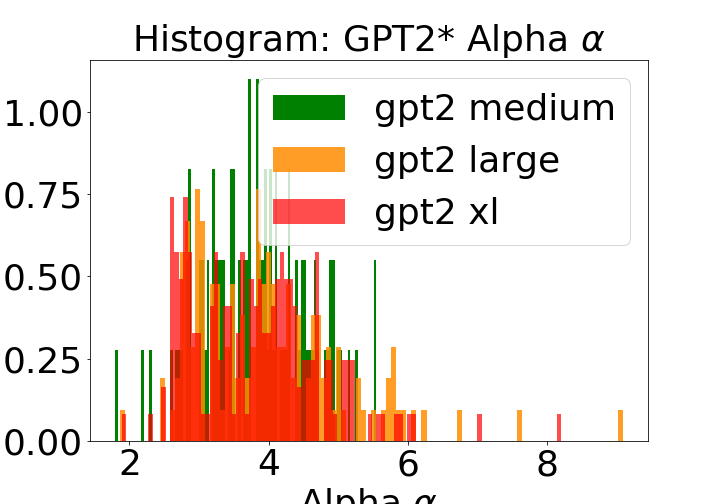
\includegraphics[width=5.5cm]{img/GPT2*_fnl_alpha_hist.png}
        \label{fig:gpt2-alpha-hist}
    }
    \quad
    \subfigure[Log Alpha Norm]{
        \includegraphics[width=5.5cm]{img/GPT2*_fnl_log_alpha_norm_hist.png}
        \label{fig:gpt2-pnorm-hist}
    }
    \caption{Histogram of PL exponents 
             %($\alpha$)
             and Log Alpha Norm 
             %($\log\Vert\mathbf{X}\Vert_{\alpha}^{\alpha}$) 
             for weight matrices from models of different sizes in the GPT2 architecture series.  (Plots omit the first 2 (embedding) layers, because they are normalized differently giving anomalously large values.)
             }
    \label{fig:gpt2-histograms}
\end{figure}
